\documentclass[BSc]{abdnthesis}

%% For citations, I would recommend natbib for its
%% flexibility, particularly when named citation styles are used, but
%% it also has useful features for plain and those of that ilk.
%% The natbib package gives you the following definitons
%% that extend the simple \cite:
%   \citet{key} ==>>                Jones et al. (1990)
%   \citet*{key} ==>>               Jones, Baker, and Smith (1990)
%   \citep{key} ==>>                (Jones et al., 1990)
%   \citep*{key} ==>>               (Jones, Baker, and Smith, 1990)
%   \citep[chap. 2]{key} ==>>       (Jones et al., 1990, chap. 2)
%   \citep[e.g.][]{key} ==>>        (e.g. Jones et al., 1990)
%   \citep[e.g.][p. 32]{key} ==>>   (e.g. Jones et al., p. 32)
%   \citeauthor{key} ==>>           Jones et al.
%   \citeauthor*{key} ==>>          Jones, Baker, and Smith
%   \citeyear{key} ==>>             1990

\usepackage{natbib}
%\usepackage[round,colon,authoryear]{natbib}
\setlength{\bibsep}{0pt}
\bibliographystyle{plain}
%\bibliographystyle{apalike}

\usepackage[T1]{fontenc}

% my packages
\usepackage{csquotes}

\usepackage{color}

\usepackage{tikz}
\usetikzlibrary{shapes.geometric, arrows}

\usepackage{hyperref}
\hypersetup{colorlinks, citecolor=black, filecolor=black, linkcolor=black, urlcolor=black}

\usepackage{enumitem}
\setlist[itemize]{noitemsep, topsep=0pt}

% my commands
\newcommand{\nocontentsline}[3]{}
\newcommand{\tocless}[2]{\bgroup\let\addcontentsline=\nocontentsline#1{#2}\egroup}

\title{An argumentation-based approach to summarizing discussions}
\author{Charlie Egan}
% IMO this is a bit silly, but some like to include these. To remove,
% delete this declaration and remove the option from the
% \documentclass definition above.
%\qualifications{PhD, Computer Science, University College London, 1997\\%
%BEng (Hons.) Electrical and Electronic Engineering, The University of Wales, Swansea, 1992}
\school{Department of Computing Science}

%%%% In the final submission of a thesis, this should only be the year
%%%% of submission.  However, it is useful to use \date{\today} for drafts so that
%%%% they don't get mixed up.

\date{2016}

%% It is useful to split the document up as chapters and include
%% them.  LaTeX will sort out all the numbering and cross-referencing
%% for you --- if you run it enough times!

%% If you want to include only a couple of chapters then use the
%% \includeonly{} command with a list of the file/chapter names that
%% you wish to include.  NB, this must be in the preamble.

\def\sfthing#1#2{\def#1{\mbox{{\small\normalfont\sffamily #2}}}}

\sfthing{\PP}{P}
\sfthing{\FF}{F}

%% This will make sure that all cross-references are correct (including
%% references to those file not included) but will produce a dvi
%% file with only those files/chapters you specify included.

\begin{document}

%%%% Create the title page and standard declaration.

\maketitle
\makedeclaration

%%%% Then the abstract and acknowledgements

\begin{abstract}
  With an ever increasing number of internet users, online communities are hosting an increasingly large number of discussions. This user generated content contains millions of statements, opinions and ideas. Our systems for discovery of such information are playing catch-up and in the meantime much of this resource is lost.

  In this paper an approach for summarising such information is proposed. Our approach is based on the idea of `point extraction', where a point is a verb and it's associated arguments. We implement and test our approach on six online debates before evaluating our summaries against a baseline. We found that we were able to improve significantly on the baseline summaries of the same debate.
\end{abstract}

\begin{acknowledgements}
  \begin{itemize}
    \item{Adam \& Advaith}
    \item{Parents}
    \item{Department}
  \end{itemize}
\end{acknowledgements}

%%%% It should have a table of contents, but delete the other two as
%%%% necessary.

\tableofcontents
%\listoftables
%\listoffigures

\chapter{Introduction\label{chap:introduction}}
  More people are online than ever before. Comment threads and forums allow us to spend our spare time participating as contributors - rather than just consumers consumers. From the latest blockbuster title to yesterday's celebrity misdemeanor there's an online conversation already well underway.

  These discussions, where statements are encoded in natural language, represent a large untapped resource of ideas and opinions. A higher level view of this ever-evolving `data set' would be of interest to many working the social sciences as well as the participants of online discussions.

  This project explores an approach for summarization of such information. At the core of the approach is the notion of a `point' - a short refined argument statement. An argument is made up of a number of points and we are going to use these as our content units in our summarization task. Points are extracted from text and grouped to give a summary of the discussion. We test our implementation's performance by running an evaluation using summaries generated from various political debates sourced from online discussions \cite{walker2012corpus}.

  \section{Motivation}
    ``A summary can be loosely defined as a text that is produced from one or more texts, that conveys important information in the original text(s), and that is no longer than half of the original text(s) and usually significantly less than that.'' \cite{radev2002introduction}

    Summarization has been a long-running task in the field of Natural Language Processing. Summarization sub-tasks such as extraction and compression, where text is selected and removed to arrive at a summary, have become commonplace due to the complexities introduced by abstractive methods. Extractive methods for this have become largely statistical using Naive-Bayes \cite{kupiec1995trainable} approaches and, more recently, Neural Networks \cite{svore2007enhancing}.

    Argumentation Mining, a newer area of study, has the aim of detecting argumentative discourse structure in text. Argumentation Mining has been successfully used in the processing of formal texts such as parliamentary records \cite{palau2009argumentation} and legal documents (cite: Semantic Processing of Legal Texts) where arguments are often stated more explicitly. However, Argumentation Mining has also more recently been applied to more informal text \cite{park2015conditional}. Such applications, coupled with summarization, encapsulates much of the idea for this project.

    The points idea was adopted from a previous project from the department that used points in a system for stance classification. This had point identification, however, the tool was not capable of extracting units of text smaller than sentences. The tool was capable of linking contrasting points, but could only make matches based on the present of negation terms.

    The project was based on the concept of a point as well as the idea that informal argumentative discourse could be used to build a high-level summary of an online discussion. News article comment sections; forum threads; film \& product reviews and even extended email conversations are all candidate applications for such a tool.

  \section{Objectives}
    Starting with the definition for a point: a verb and it's dependents, we set the following objectives for the project.

    Leading on from the stance classification project (cite Angrosh?), we wanted to improve on the extraction of points from text. This meant ensuring a complete list of a verb's dependents was maintained for presentation for a given point - rather than just using the containing sentence.

    Another goal was to investigate relationships between points such as contrastive or co-occurring points - this involved expanding the ways in which related points could be matched, beyond negation. As secondary objective, we wanted to investigate supporting points. These were points that not only commonly co-occured in posts but also had a place in an argument structure.

    The task of stance classification was also discussed. Another secondary objective was to investigate if certain points were representative for a given known stance. Stance was annotated on some of the corpus debates.

    Finally we set out to present this information in in a way that was easy to interpret. This `presentation form' evolved into our debate summaries.

\chapter{Background \& Related Work\label{chap:background-related}}
  \section{Background}
    This project is built on existing technologies and research. This section gives an overview of the key foundations.

    \subsection{Automatic Summarization}
      ``A summary can be loosely defined as a text that is produced from one or more texts, that conveys important information in the original text(s), and that is no longer than half of the original text(s) and usually significantly less than that.'' \cite{radev2002introduction}

      Approaches to summarization could be grouped loosely into two groups, extractive and abstractive. Extractive summaries are constructed using content found in the source text. Abstractive summaries generate the summary content by performing some form of analysis on the source text. One might also group summarization tasks based on the nature of the source text. Approaches tend to summarize either single or multiple documents.

      This project is more closely related to the summarization of multiple documents, however, it applies both elements of extraction and abstraction.

      \subsubsection{Multi-document Summarization}
        Summarizing text made up of documents from different authors poses an interesting challenge. Using multiple documents introduces repetition and contradictions - this makes selection tasks such as extraction and compression more complex.

        Earlier work on multi-document summarization suggested the task was going to require an abstractive approach \cite{McKeown1999TMS315149315355}. The justification being that extraction techniques used for single document summaries, not being able to connect information between documents, would lead to incoherent and repetitive summaries. An alternative approach clustered paragraphs on the same topic from multiple documents and then use natural language generation techniques to combine phrases from paragraphs into a coherent summary \cite{McKeown1999TMS315149315355}. A similar approach creates clusters by parsing sentences and using predicate-argument structures to link phrases \cite{barzilay1999information} (comment about being similar to our points extraction and grouping?). Interestingly, while both rely methods rely on natural language generation, neither use a semantic representation.

        More recently, MEAD, a centroid-based, multi-document summarization tool has been able to produce good summaries without abstraction and generation \cite{radev2000centroid}. Compared to previous abstractive systems such as SUMMONS that relied on templates \cite{mckeown1995generating}, MEAD was more generally applicable.

        Most work on the summarization of multi-document sources has focused on news articles. While there are parallels between this and the summarization of online discussion, fundamentally they are different tasks. More closely related to this project is opinion mining.

        Opinion mining or sentiment analysis is an approach often applied to user reviews, documents discussing a product or service. Early work in the area focused on the problem as a classification task, categorizing documents based on their sentiment bearing terms \cite{turney2002thumbs}. More recently there as been a greater focus on aspect-based approaches that attempt isolate sentiment terminology to specific topics such as product features \cite{hu2004mining}.

      \subsubsection{Sentence Compression \& Content Unit Size}
        While sentences are often the default `content unit' used in extractive summarization, often smaller units are more desirable. Sentences found in real documents and discussions can make a number of statements each of which can be useful when creating a summary. Sentences may also include surplus information. In this case sentences can be compressed statistically, in a similar way to documents are in extractive summarization.

        Both noisy channel and decision based models have used on parsed sentences for the task of sentence compression \cite{knight2000statistics}. Our approach for compression where points are extracted around a verb, does not seem to have been previously documented.

        (comment that the largest coherent unit is a sentence in an extractive summary, even that might not be right (bad grammar, co-referring expressions). Reference: Ultra-Summarization: A Statistical Approach to Generating
        Highly Condensed Non-Extractive Summaries)

      \subsubsection{Evaluation of Summaries}
        The evaluation of automatically generated summaries is an ongoing discussion. A common approach is to make a comparison against a model summary, typically written by a human. Various metrics such as ROUGE \cite{lin2004rouge} are used to make the comparison between summaries statistically. These are however limited by the assumption that there is a single best model for a summary. Alternative methods have been proposed. The Pyramid Method is one such example, it models content units across the collection of summaries being evaluated to give each content unit a weight based on how commonly it occurs \cite{nenkova2004evaluating}. These weights are used to allocate scores to summaries without an ordering bias.

        Automated methods are used primarily at the Document Understanding Conference when many summaries must be evaluated for a given task. Ideally however summaries could be manually evaluated. This would allow extrinsic attributes such as the utility of a summary for a particular task to also be accounted for. (reference to SUMMAC?, automated http://citeseerx.ist.psu.edu/viewdoc/summary?doi=10.1.1.13.489)

        In this project we compare our summaries against those generated using the approach outlined here \cite{nenkova2006compositional} as a baseline.

    \subsection{Argumentation Mining}
      Argumentation Mining is a task that involves the identification components of arguments within text such as premises and the conclusion. The task also often involves fitting these components into a template or known pattern to enable some form of reasoning. \cite{palau2009argumentation}

      A relatively new research area - combining ideas from natural language processing, information extraction and argumentation theory - argumentation mining is based largely on discourse  theory. While argumentation mining can be applied to structured text (source?), ultimately mining of free text is the goal. This means that argumentation tools often need to model concepts from linguistic research such as rhetoric structure theory \cite{mann1988rhetorical} and local coherence centering \cite{weinstein21centering}.

      \subsubsection{Identifying Argumentative Structures in Text}
        When identifying argumentative structures in text the first step is often to classify phrases that are part of an argument being made. One of option is to define rules for argumentative sentences or clauses. This can also be approached as a classification task, statistical methods such naive-bayes have also been used \cite{palau2009argumentation}. The result of this stage is a collection of unrelated clauses potentially spanning many arguments present in the source text.

        The next stage in the analysis is to group identified units together into separate arguments. While sometimes the document's structure (chapters and sections) can be used to inform the grouping task this is hard to make generally applicable. Documents are rarely consistently formatted and arguments will often span many sections. Other options include grouping based on the similarity of the unit contents - presence of certain words etc. \cite{palau2009argumentation}

        Once identified units have been grouped into different arguments it becomes possible to start looking into the argument's structure. Different units need to be classified as either premises or conclusions - this can again be approached as a classification task \cite{palau2009argumentation}. Once such as structure for the units has been established it's possible to do analysis this connected structure such as identifying supporting claims for conclusions.

        A further task is relating arguments within the document to one another, this is a far more challenging task. Fitting the argument structure to allowed patterns defined by a context-free grammar is one proposed approach \cite{palau2009argumentation}.

    \subsection{Dependencies}
      The approach implemented as part of this project relies on the products of research in the following areas.
      \subsubsection{Topic Modeling}
        Topic modeling covers a set statistical modeling techniques used to identify and group `topics' in text. Fundamentally, this involves looking for words that are relatively more common on one document vs a more general corpus. Documents often contain multiple topic words that need to be grouped into more conceptual topics. One approach to this is is Latent Dirichlet Allocation (LDA), this implements a "three-level hierarchical Bayesian model" \cite{blei2003latent} and is the approach used for topic modeling in this project.
      \subsubsection{Dependency Parsers}
        Parsing text for dependencies involves building upon a phrasal parse to extract relations between tokens in text. Dependencies are identified using rules applied to phrase structure trees. Various dependency parsers exist, this project makes use of the dependency parser included as part of the Stanford CoreNLP framework \cite{de2006generating} which is based on their probabilistic context-free grammar phrasal parser \cite{klein2003accurate}. The rules used in the Stanford dependency parser based on ``Universal Stanford Dependencies" \cite{de2014universal}.
      \subsubsection{Querying Dependency Parses}
        To make use of the dependency parse a means of querying the graph is required. \textit{Semgrex} is one such approach, this defines a regular expression style syntax for expressing queries on nodes and relations in a dependency graphs \cite{Chambers2007}. More generally however, the task about querying nodes and edges in a directional graph. For this project we opted to use \textit{Cypher}\footnote{http://neo4j.com/docs/stable/cypher-introduction.html}, the graph query language implemented by the \textit{Neo4j}\footnote{http://neo4j.com/} graph database. This was chosen for the querying of dependency parses because it allowed many separate graphs to be queried in parallel for the same pattern using a more familiar declarative syntax.

  \section{Related Work}
    Having covered the technologies and areas of research that underpin this project I will now discuss similar work that come closer to combining these different areas, as this this project does.

    Summarizing discussions, email and meetings

    Summarizing online and archived discussions

    Summarizing opinions on online discussions

    Argumentation in online discussions

    Argumentation driven summaries not been covered. (Result of the review of related work is that:  there does not appear to have been any work that approaches the summarization of discussion from an argumentation mining perspective.)

  \section{Motivation}
    Round up why our project is different and interesting

\chapter{Technologies\label{chap:technologies}}
  Our project relies on a number of software dependencies, these act as a foundation to services we implemented.

  \tocless\section{CoreNLP}
    \blockquote{Stanford CoreNLP provides a set of natural language analysis tools.}\footnote{https://stanfordnlp.github.io/CoreNLP/}

    CoreNLP provides the basis for our points extraction analysis and assists in selecting extracts during the generation of summaries. Running as a separate service, modules in our analysis pipeline make requests to get sentences, dependency parses and lemmas for text. While the CoreNLP frame work implements a number of different `annotators', we only make use of \texttt{depparse} \& \texttt{lemma} --- which depend on \texttt{tokenize}, \texttt{ssplit} and \texttt{pos}.

  \tocless\section{Verb Case Frames}
    While not strictly a software dependency, we made use of verb cases frames (standard representations of allowed verb argument patterns) in the definition of valid points. Using FrameNet frames included as part of the VerbNet index \cite{schuler2005verbnet, fillmore2002framenet}, we were able to implement a mapping between these and the dependency parse information. This connection was implemented using queries on the Neo4j graph database.

  \tocless\section{Cypher and Neo4j}
    \blockquote{Neo4j is a highly scalable native graph database that leverages data relationships as first-class entities, helping enterprises build intelligent applications to meet today's evolving data challenges.}\footnote{http://neo4j.com/}

    We use Neo4j to store parse information. Sentences are parsed using the CoreNLP dependency parser and the resulting graph structure is saved to a Neo4j instance. Tokens and dependencies are represented as nodes and edges respectively. Nodes are used to store the token in plaintext; the lemma, part-of-speech tag and its index in the source sentence. Edges are directional; connect governor to dependent tokens; and have a single attribute to store the dependency type.

    \blockquote{Cypher is a declarative graph query language that allows for expressive and efficient querying and updating of the graph store.}\footnote{http://neo4j.com/docs/stable/cypher-introduction.html}

    Cypher is used to query dependency parses stored in the Neo4j database. After parsing the sentences from a user's post, all the dependency parses are saved. At this stage, a series of Cypher queries are executed to filter for allowed point patterns. These patterns, derived from case frame information, are represented in the Cypher syntax. Using Neo4j and Cypher in this way allows points to be extracted from many sentences at once. This was key to completing the analysis of large discussions in reasonable time.

  \tocless\section{Latent Dirichlet Allocation Implementation\label{sec:lda-tech}}
    We use a service to evaluate the core topics of a discussion. This is based on an implementation of the \textit{Latent Dirichlet Allocation} generative model\footnote{https://github.com/ealdent/lda-ruby}. Discussion text is analyzed as a whole by a \textit{Topic Analyzer}, the service that exposes this implementation to other components --- see Chapter \ref{chap:system-architecture}. Topics are used in accessing the value of extracted points as well as guiding the extraction process.

  \tocless\section{ERB}
    \blockquote{ERB provides an easy to use but powerful templating system for Ruby}\footnote{http://apidock.com/ruby/ERB}

    We use ERB (Embedded RuBy) to generate HTML documents used as part of the evaluation (see Chapter \ref{chap:evaluation}). ERB templates were defined for each summary style being evaluated. The evaluation forms distributed on Mechanical Turk were also generated using ERB. Having templates for these documents allowed sets of summaries and surveys to be consistently re-generated as we iterated on the functionality of the summarization module and format of the questionnaires.

  \tocless\section{Ruby \& Go}
    Almost all of the functionality of the tool is implemented in the Ruby programming language. Ruby was selected for its familiarity as well as its suitability in connecting multiple networked services together. Once points had been extracted using a Ruby service, making use of CoreNLP and Neo4j, points are curated using a small program written in Go, this task required fast iterations and it allowed the results of changes to the point curation to be reviewed in a faster feedback cycle. Point curation is discussed in chapter \ref{chap:point-curation}.

  \tocless\section{Docker}
    \blockquote{Docker allows you to package an application with all of its dependencies into a standardized unit for software development.}\footnote{https://www.docker.com/what-docker}

    Docker is used to isolate the different environments of each service. CoreNLP and Neo4j are both run as containers using standard images. Our modules are run under the same system. All modules in communicate using JSON requests. Docker Compose is used to codify the system's configuration and start services when they are required for use in development.

  \tocless\section{git}
    All work for the project, including documentation, was tracked in version control using git. Changes were synced with a remote repository on GitHub and other remotes as a means of backup and transfer between machines.

\chapter{Research Goals\label{chap:res-goals}}
  Having justified working on a project in the area I will now look to given an overview of the project's research goals. We set out to investigate the following sub tasks.

  \section{Using \textit{Points} as a content units}
    \subsection{Extracting all verb dependencies}
      Something that was missing from the previous project was\dots
  \section{Point clustering}
    \subsection{Identification of Contrastive Points}
  \section{Generating Point Summaries}
    interface to inspect the results of the analysis for the debate
  \section{Modular architecture to enable experimentation}

\chapter{System Architecture\label{chap:system-architecture}}
  This chapter is intended to give a technical overview of the system design and add context to the analyses detailed in the following chapters. The system has been implemented as a series of isolated modules that together form a processing pipeline. Each stage can take a significant time to complete, so the output is written to disk in standard format between each stage. In summary, extracted points are aggregated for an entire debate, these are then revised before being grouped into a summary.

  \begin{figure}[!h]
    \centering
    \begin{tikzpicture}[node distance=3.5cm]
      \node (agg) [service] {Aggregator};
      \node (top) [service, left of=agg] {Topic Analyzer};
      \node (ext) [service, above of=agg, yshift=-1.5cm] {Extractor};
      \node (cur) [service, right of=agg] {Curator};
      \node (sum) [service, right of=cur] {Summarizer};
      \node (cor) [extservice, above of=sum, yshift=-1.5cm] {CoreNLP};
      \node (neo) [extservice, above of=ext, yshift=-1.5cm] {Neo4j};

      \draw [flow] (agg) -- (cur);
      \draw [flow] (cur) -- (sum);
      \draw[dotted] [depends] (agg) -- (ext);
      \draw[dotted] [depends] (ext) -- (neo);
      \draw[dotted] [depends] (ext) -- (cor);
      \draw[dotted] [depends] (sum) -- (cor);
      \draw[dotted] [depends] (top) -- (agg);
    \end{tikzpicture}
    \caption{\\Architecture Diagram. Arrows represent the pipeline data flow; dotted lines represent dependencies.}
    \label{fig:arch-dia}
  \end{figure}

  Figure \ref{fig:arch-dia} shows a high-level overview of the various modules and how they make up the analysis pipeline. Points for all posts in the source text are gathered by the \textit{Aggregator}; these are filtered and cleaned by the \textit{Curator}, and finally, curated points are used to generate a summary by the \textit{Summarizer}.

  Before source text can be analyzed it must be cleaned for invalid characters. Posts in a discussion begin as single text files, these are loaded and transformed into JSON files that preserve their index and valid UTF-8 content. The \textit{Aggregator} loads these JSON post files to extract the points made in each post.

  The \textit{Aggregator} loads all the JSON posts for the selected discussion. Before extracting points for each in turn it uses the text from all the posts (representing the discussion) to collect a list of topic words from the \textit{Topic Analyzer}. For each post in turn the text and topics\footnote{Only sentences containing a topic word are analyzed for points to reduce processing time.} are submitted to the \textit{Extractor}. This carries out the point extraction process for each sentence in the post --- making use of both the CoreNLP dependency parser and Neo4j datastore (described in detail in Chapter \ref{chap:point-extraction}). Then extracted points for all posts are saved to disk. A modern, mid-range computer can complete 150,000 words spread across 2300 posts in around 10 minutes, this is the slowest stage of the analysis pipeline.

  While points must come from a sentence containing a topic word, at this stage points are still largely unfiltered. The \textit{Curator}, a short program to filter and re-format points makes a series of transformations such as merging pronouns under a single \texttt{PERSON} label. Patterns for low-quality points are also encoded at this stage, for example: the \texttt{PERSON.nsubj be.verb sure.adj} point pattern that comes from every ``\textit{I'm sure}''; is rejected. These transformations and rejections are applied to the list of points and a refined version is saved for use at the next stage.

  The \textit{Summarizer} is the final stage in the pipeline. Given a list of curated points, this module groups common points into the different summary sections. Sections are filled using points that have not been used earlier in the summary and are suitable for the current group. Once a point has been used in a summary section, it cannot be used again. This module must also choose an extract to display for each point. The point \texttt{abortion.nsubj be.verb right.dobj} occurs many times in the discussion and a single occurrence to represent this must be selected. This process makes use of the CoreNLP module again to request a dependency parse used in rating the quality of extracts. Selected extracts are formatted and used as text seen in summaries.

  The \textit{Summarizer} formats the grouped extracts for selected point patterns as summary HTML files. This is the end of the pipeline - possibilities for further work are discussed in Chapter \ref{chap:conclusion}.

  A monolithic architecture was avoided due to processing time required at each stage. Running the entire process, when making adjustments at the final stage, was not feasible. Currently stages in the pipeline must be run manually --- however this is trivial to automate with a script. The process for using the pipeline has been outlined in the Maintenance Manual in Appendix \ref{app:maintain}. The following chapters build on this technical overview and give more detail on the intricacies of the analysis performed by each module.

\chapter{Point Extraction\label{chap:point-extraction}}
  \section{Point Concept Overview and Examples}
    A `point' is a concept we created to describe a common object in our analysis --- originally defined as: a verb and its arguments. Points encapsulate both a human-readable extract from the text as well as a pattern representing the core components that can be used to match and compare points to others. Extracts and patterns are stored as attributes in a key-value structure that represents a point. Lets walk through extracting such a structure from the following sentence:

    \smallskip
    \begin{center}
      \blockquote{\textit{I don't think so, an unborn \textbf{child} (however old) \textbf{is} not yet a \textbf{human} being.}}
    \end{center}
    \smallskip

    This sentence puts forward the idea that, until a baby is born, it does not qualify as human. This idea is centered around the verb `\textit{is}', \blockquote{...an unborn child \textbf{is} not yet a human being}. Another sentence in the discussion may also put forward this idea, for example: \blockquote{\textit{So you say: children are not complete humans until birth?}}. Both of these sentences have words that express the same idea only the context differs. At this first stage, negation and question tokens are ignored. The aim is to get to the core idea being discussed, regardless of negation or what might be implied by a question. We represent these core ideas as point patterns which list the key arguments and the verb. These two sentences both contain points with the pattern: \texttt{child.subject be.verb human.object} --- the core idea that they both make reference to.

    This pattern loses some of the sentence context and is not suitable for use in human-readable text. To overcome this, when extracting points from sentences, points are represented as a pattern but \textit{with an accompanying extract}. Extracts are strings made of one or more sentence substrings. The extracts for the points in these two sentences would be:

    \smallskip
    \begin{center}
      \blockquote{\textit{an unborn child is not yet a human being}} \\ \blockquote{\textit{children are not complete humans until birth?}}
    \end{center}
    \smallskip

    Using this pattern/extract representation enables points expressed in different tenses and contexts to be grouped together using their patterns --- while also retaining the relevant parts of the sentence to present the human-readable points. While points are the fundamental unit used in our analysis, Figure \ref{fig:discmod} shows how points make up part of a larger, hierarchical, discussion model. Points are stored in a key value representation with attributes for the pattern, extract, verb and point's original source post in the discussion, see Table \ref{tab:point-keyval}.

    \begin{figure}
      \centering
      \caption{Discussion model showing relationships between subcomponents}

      \TBox[fill=black!5]{10cm}{
        Discussion \\[1ex]
        \TBox[fill=black!10]{9.7cm}{
          Post \\[1ex]
          \TBox[fill=black!15]{9.4cm}{
            Sentence \\[1ex]
            \TBox[fill=green!5]{9.1cm}{
              Point \\[1ex]
              \TBox[fill=green!15]{2.5cm}{
                Pattern \\[1ex]
                \TBox[fill=green!25]{2.2cm}{Component}
              }
              \TBox[fill=green!15]{1.68cm}{Extract}
              \TBox[fill=green!15]{1.68cm}{Verb}
              \TBox[fill=green!15]{1.68cm}{Source}
            }
          }
        }
      }
      \label{fig:discmod}
    \end{figure}

    \begin{table}[]
      \centering
      \caption{Example point data structure}
      \label{tab:point-keyval}
      \begin{tabular}{|l|l|}
        \hline
        \textbf{Attribute}       & \textbf{Example Value}                         \\ \hline
        Pattern                  & \texttt{\{child.nsubj be.verb human.dobj\}} \\
                                 & Single Component: \texttt{child.nsubj}         \\ \hline
        Extract                  & ``\textit{an unborn child is not yet a human being}''               \\ \hline
        Verb                     & to \textit{be}                               \\ \hline
        Source                   & \textit{Post: \#x42, Debate: Abortion}          \\ \hline
      \end{tabular}
    \end{table}

    The \textit{Pattern} attribute consists of a list of two or more \textit{Components}. Each component represents a dependency of the verb and the relation of that dependency. For example, if a child were to be the subject, then the component would be \texttt{child.nsubj} (nominal subject). Relations are defined using Universal Stanford Dependencies\footnote{http://universaldependencies.org/docs/en/dep/}. Patterns are broken down into components to enable certain comparisons between points, for example, to test that \texttt{abortion.nsubj be.verb \textbf{legal.dobj}} and \texttt{abortion.nsubj be.verb \textbf{illegal.dobj}} are counter points.

    With a definition for a point we can now explore the process of extracting these from text. A point, as described above, is built up using information from a dependency parse. A dependency parse is represented in a graph structure showing relationships between different tokens.

	\begin{center}
      \begin{dependency}[edge horizontal padding=0]
          \begin{deptext}
              A \&[2cm] fetus \&[2cm] has \&[2cm] rights \&[0.5cm] . \\
          \end{deptext}
          \depedge{2}{1}{determiner}
          \depedge{3}{2}{nominal subject}
          \depedge{3}{4}{direct object}
          \depedge{3}{5}{punctuation}
          \deproot[edge unit distance=2.1ex]{3}{verb}
      \end{dependency}
	\end{center}
    \vspace{-7mm}

    From this parsed representation of the sentence we can see how both an extract \blockquote{\textit{A fetus has rights.}} and pattern \texttt{fetus.nsubj have.verb right.dobj} could be constructed using the graph's relations. In this example the nominal subject and direct object relations form the pattern, while all relations are followed from the verb to generate the extract. In more complex graphs not all relations are used to avoid excessively long extracts. Also, patterns must sometimes be derived from more than subject and object relations. Sentences often contain more than one point, the following (more complex) dependency parse shows a sentence that references two different points.

    \vspace{3mm}
	\begin{dependency}[edge horizontal padding=0]
		\begin{deptext}
			A \&[0.7cm] baby \&[0.7cm] has \&[0.7cm] rights \& , \& so \& a \&[0.7cm] fetus \& also \&[0.7cm] has \&[0.7cm] rights \\
		\end{deptext}
		\depedge{2}{1}{det}
		\depedge{3}{2}{nsubj}
		\deproot{3}{verb}
		\depedge{3}{4}{dobj}
		\depedge{3}{5}{punct}

		\depedge[edge unit distance=1.2ex,label style={fill=green!15}]{3}{10}{parataxis}

		\depedge{8}{6}{advmod}
		\depedge{8}{7}{det}
		\deproot{10}{verb}
		\depedge{10}{8}{nsubj}
		\depedge{10}{9}{advmod}
		\depedge{10}{11}{dobj}
	\end{dependency}
    \vspace{-2mm}

    Here the parse information helps isolate the two points: \texttt{baby.nsubj have.verb right.dobj} and \texttt{fetus.nsubj have.verb right.dobj}. A \texttt{parataxis} relationship connects the two --- though this is one such relation that is not used to expand a point's extract.

  \section{Defining Points with Verb Frames}
    Not all of a verbs relations should be included in the point pattern but rather only those essential to the meaning. This typically means using only subject and object; however, this cannot be defined for all verbs with a single rule. Some additional dependencies, like adverbial modifiers and parataxis as seen in the previous example, which do not introduce information relevant to the point's pattern can be universally excluded. However, not all dependency types are easily classified. This is largely due to the different verb classes (transitive, intransitive and ditransitive) and how these are represented in parses by the CoreNLP parser. In order to look for legal patterns in dependency parse graphs, we needed an index of verb transitivities that listed allowed patterns for a given verb. We started using FrameNet frames for this task and later extended these with a generic query as a heuristic to match patterns not present in FrameNet.

    \tocless\subsection{VerbNet and FrameNet}
      VerbNet is an XML verb lexicon that lists classes of verbs and accompanying FrameNet frames \cite{schuler2005verbnet,fillmore2002framenet}. Represented in VerbNet's 274 `classes' are 4402 member verbs. For each of these verbs classes, a wide range of attributes are listed. FrameNet frames are one such attribute, and the only one we make use of. These describe the verb's syntactic arguments and the semantic meaning of each in that frame. We can use the frames represented in the source class to determine the allowable forms for each verb. An example frame for the verb `murder' is shown in Figure \ref{fig:murder-frame}. Here we see that the verb takes two Noun Phrase arguments, an Agent (murderer) and Patient (victim).

      \begin{figure}
        \centering
        \caption{VerbNet frame example for verb murder}

        \begin{minted}{XML}
<FRAME>
  <DESCRIPTION primary="NP V NP" secondary="Basic Transitive"/>
  <EXAMPLES><EXAMPLE>Brutus murdered Julius Cesar.</EXAMPLE></EXAMPLES>
  <SYNTAX>
    <NP value="Agent"><SYNRESTRS/></NP>
    <VERB/>
    <NP value="Patient"><SYNRESTRS/></NP>
  </SYNTAX>
  <SEMANTICS>...</SEMANTICS>
</FRAME>
        \end{minted}
        \label{fig:murder-frame}
      \end{figure}

      We use this \texttt{SYNTAX} element information to determine the type of dependencies that can be included in the pattern for a given verb. To create a `verb index' we parsed the VerbNet catalogue into a key-value structure where each verb was the key, and the list of allowed frames the value. Some verbs are listed in more than one class; for example, \textit{feel} is listed in seven classes. In such cases the verb was allocated all frames for all classes it was a member of. Using this index, points can be extracted by querying the verb's dependency parse using information from each of its frames.

    \tocless\subsection{Matching Frames in Parses}
      With an index of verbs and their allowed frames, all the information required to identify points in dependency parses is available. However, frames are not inherently capable of querying the dependency graph structure and queries for each type of frame must be written. While frames in different categories encode additional semantic information, there are far fewer `syntactically unique' frames than verb classes. Common frames such as \texttt{NounPhrase Verb NounPhrase} cover a high percentage of all frames in the index. We have manually implemented a means of querying dependency parses for 17 of the more common patterns covering 96\% of all frames in the index.

      FrameNet provides short example sentences for each frame. Using the dependency parses for these examples (returned from CoreNLP), we were able to manually map dependency relations to the syntax components in the frames. Mapping \texttt{nsubj} and \texttt{dobj} relations to noun phrases is relatively straight forward. However, more complex frames such as \texttt{NP VERB NP PREP NP PREP NP} require a mapping from a complex, recursive parse onto a flat frame structure. In these more complex cases, queries must search beyond the verb's immediate arguments for tokens with relations matching these additional frame components. For example, in the \texttt{NP VERB NP PREP NP PREP NP} frame, the first prepositional is connected with a case relation to the third noun phrase; which is in turn connected to the verb via a nominal modifier. Frames are always flat and nested structures must be expressed in the queries to flatten parses for these larger frames.

      These queries, mapping frames to parses, must be written manually and was a time consuming exercise. Queries are written in \textit{Cypher}, the declarative query language implemented by the Neo4j database that we used to store dependency parses during analysis. Figure \ref{fig:npvnpquery} shows an example for a simple frame. Restrictions imposed commonly require subject and object relations. The query returns the nodes that match these relations. Should a verb \textit{not} have the relations to complete the frame then nothing is returned from the query.

      \begin{figure}
        \centering
        \caption{Example Cypher query for the common \texttt{NP V NP} frame}

        \begin{minted}{Cypher}
MATCH (verb:Node)
WHERE verb.uuid = UUID
MATCH (verb)-[rel_nsubj:REL]->(nsubj:Node)
MATCH (verb)-[rel_dobj:REL]->(dobj:Node)
WHERE rel_nsubj.label = "nsubj"
AND rel_dobj.label = "dobj"
RETURN nsubj, verb, dobj;
        \end{minted}
        \label{fig:npvnpquery}
      \end{figure}

      The remaining 4\% of frames, as well as verb cases not covered by FrameNet, were matched using a `Generic Frame' - discussed in the following section.

    \tocless\subsection{The Generic Frame}
      Originally our intent had been to use only queries derived from FrameNet frames to define allowed patterns for points. However, there were verbs missing frames for some patterns of interest. Usually this meant a simple frame for the verb was listed but it failed to adequately capture point idea. Take the following example:

      \bigskip
      \begin{center}
        \blockquote{\textit{These images reflect the reality of abortions}}
      \end{center}

      This is an extract that only matched \texttt{image.nsubj reflect.verb}. Shorter points like this make extracts for points in a cluster considerably more varied, resulting in less cohesive clusters. To overcome this we introduced the idea of the `Generic Frame'. This was a new query that could be run against any dependency graph to extract subjects, objects and open clausal complements. This was used to increase the number of complete points. For the extract above, the Generic Frame matched this more complete pattern: \texttt{image.nsubj reflect.verb reality.dobj}.

    \tocless\subsection{Copula Verbs}
      The dependency parse differs for copula verbs as the verb is no longer the root of the parse. Analyzing dependencies \textit{from the verb} only works when the verb is the root. The following examples illustrate the inherently different structure.
      \begin{multicols}{2}
        \raggedcolumns
        \begin{center}
          \begin{dependency}[edge horizontal padding=0]
            \begin{deptext}
              women \&[0.5cm] have \&[0.5cm] rights \\
            \end{deptext}
            \depedge{2}{1}{nsubj}
            \depedge{2}{3}{dobj}
            \deproot[edge unit distance=2.3ex]{2}{root}
          \end{dependency}
        \end{center}
        \columnbreak
        \begin{center}
          \begin{dependency}[edge horizontal padding=0]
            \begin{deptext}
              fetuses \&[0.5cm] are \&[0.5cm] people \\
            \end{deptext}
            \depedge{3}{1}{nsubj}
            \depedge{3}{2}{cop}
            \deproot[edge unit distance=2.3ex]{3}{root}
          \end{dependency}
        \end{center}
      \end{multicols}

      Rather than making the copula verb the head of the sentence, we opted to write adjusted queries that could be used for copula verbs when matching against frames. This allows the dependency parse to be left unaltered and makes the implementation more explicit. The example above becomes \texttt{fetus.nsubj be.verb people.dobj} so it matches queries like: \textit{points where people are the `object'}.

  \section{Human Readable Extracts for Points}
    So far we have covered the identification of points and how the dependency parse information has been interpreted to arrive at a point's pattern. This is separate from the point extract, which is a human readable sentence that can be presented in a summary. This is extracted using a second query on the information in the dependency parse. The task of selecting an extract for a point can be described as follows: recursively follow dependencies to nodes from the verb until the tree is fully explored.

    This task was implemented as another Cypher query, similar to verb frames. However, rather than only detecting a small number of expected dependencies, this query follows all dependencies recursively. Nodes in the graph that are related to the verb, or any of its descendants, are returned as part of the extract for the point. However, to keep points succinct the following relations are prevented from extending the extract tree: \textit{adverbial clause modifiers, clausal subjects, clausal complement, generic dependencies and parataxis}. Generic dependencies occur When the parser was unable to determine the dependency type. These either arise from errors or long-distance dependencies and are rarely useful in extracts. However, the other blacklisted dependencies (csubj, ccomp etc.) were selected based on our results and should be seen as a starting point. While these often led to including unnecessary information, always excluding them is likely an oversimplification. The following dependency graph depicts the recursive extract expansion process.

    \begin{center}
      \begin{dependency}[edge horizontal padding=0]
        \begin{deptext}
          I \&[0.0cm] do \&[0.0cm] n't \&[0.1cm] think \&[0.5cm] so \&[0.1cm] , \&[0.0cm] an \&[0.0cm] unborn \&[0.1cm] child \&[0.0cm] ( \&[0.0cm] however \&[0.3cm] old \&[0.5cm] ) \&[0.1cm] still \&[0.7cm] has \&[0.2cm] rights \\
        \end{deptext}

        \depedge{4}{1}{nsubj}
        \depedge{4}{2}{aux}
        \depedge{4}{3}{neg}
        \depedge{4}{5}{advmod}
        \depedge{4}{6}{punct}
        \depedge[edge unit distance=1.2ex]{4}{15}{ccomp $\rightarrow$}

        \depedge[edge style={green!75!black, thick}]{9}{7}{det}
        \depedge[edge style={green!75!black, thick}]{9}{8}{amod}
        \depedge[edge style={red!90!black, thick}]{9}{12}{dep $\rightarrow$}

        \depedge{12}{11}{advmod}
        \depedge{12}{10}{punct}
        \depedge{12}{13}{punct}

        \depedge[edge style={green!75!black, thick}]{15}{14}{advmod}
        \depedge[edge style={green!75!black, thick}]{15}{16}{dobj}
        \depedge[edge unit distance=1.9ex,edge style={green!75!black, thick}]{15}{9}{$\leftarrow$ nsubj}

        \deproot[edge unit distance=4.0ex,edge style={green!75!black, thick}]{15}{query root}
      \end{dependency}
    \end{center}

    The green paths represent a query expanding into the graph following permitted dependencies. This gives \blockquote{\textit{an unborn child still has rights}} as the extract for the point. Upon reaching \texttt{dep}, a blacklisted dependency, that route is no longer explored and so excluded from the extract. Should the query root have been for the other verb (\textit{think}) the blacklisted clausal compliment would have isolated the extract to \blockquote{\textit{I don't think so,}}.

    This effect is not dissimilar from sentence compression, only there is a starting point `query verb'. The end result is not so dissimilar to that reported by Knight and Marcu \cite{knight2000statistics}, though the approach was fundamentally different. As they appear to do, we also strip trailing punctuation and capitalize where required. This is done at the summary generation stage in our approach, see Chapter \ref{chap:summary-generation}.

  \section{Extraction Process}
    The previous sections give a theoretical description of our points extraction approach, whereas section outlines its implementation. Making reference to Figure \ref{fig:arch-dia}, the Aggregator submits each post in turn to the Extractor. The Extractor requests dependency parses for the post text from CoreNLP before saving these into the Neo4j graph database. A query is then run to get all the verbs; for each verb the relevant frames are looked up in the index and the matching Cypher queries run to extract point patterns. For each matched verb a further query is run to extract each point's extract. These are returned as a JSON array to the Aggregator, which writes them to disk in preparation for the Curator --- the next module in the pipeline.

\chapter{Point Curation\label{chap:point-curation}}
  Points extracted at the first stage must be refined to make them suitable for use in the following summarization module. These refinements focus on removing points generated from common phrases such as `I'm sure' and `Ask yourself\dots'. While adjustments could be made as points are extracted, this is was implemented as a separate task during our implementation phase. Rejecting and editing point content is also conceptually different from identifying them in source text. Much additional information is encoded at this stage.

  \section{Minimum Requirements}
    Some basic restrictions are applied to points matched by the Generic Frame, these matches must:

    \begin{itemize}
      \item{Have a subject and object}
      \item{Contain a topic word}
      \item{Have an average word length of 5 or characters}
    \end{itemize}

    These three (opinionated) requirements balance the benefits and problems of matching a greater number of patterns, some lower quality, using the Generic Frame. This does mean that shorter points, or points without a search topic word can be returned, however, they must be matched by a FrameNet frame.

  \section{Person Nominal Subjects}
    In an effort to better cluster extracted points into distinct statements used in the discussion, we opted to merge pronouns under a single Person subject. Points with these patterns are very common but also commonly segregated by different pronouns. Take the following point patterns:
    \begin{itemize}
      \item{\texttt{people.nsubj kill.verb people.dobj}}
      \item{\texttt{he.nsubj kill.verb people.dobj}}
      \item{\texttt{they.nsubj kill.verb people.dobj}}
    \end{itemize}

    While there is a semantic difference between these points, we made the decision to amalgamate them under patterns like \texttt{PERSON.nsubj kill.verb people.dobj}. This means clusters for points are not dispersed among many pronouns. Reducing repetition between clusters means we can continue to rely on clusters size as a measure of salience in the summarization task.

  \section{Blacklists}
    To complete this module's function of cleaning and refining points, a number of `blacklists' were established. These defined patterns of components that were of little interest and should be removed.

    \tocless\subsection{Nominal Subjects}
    First points with pronoun or determiner nominal subjects were rejected. Points such as \texttt{it.nsubj have.verb rights.dobj} are ambiguous as the surrounding sentences are required to resolve the anaphor \blockquote{it}. One possible resolution was to merge such points with the most common pattern with a noun or proper noun nominal subject (\texttt{fetus.nsubj have.verb rights.dobj} for example). We opted to remove these points instead to help keep results verifiable.

      Currently the following subjects are grounds for rejection: \textit{it(PRP), that(DT), this(DT), which(WDT), what(WDT)}. Other words of the same tag such as \textit{they} or \textit{his/her} have not yet been excluded as they have yet occur as a prominent problem group. Rather than rashly remove content these are currently permitted.

    \tocless\subsection{Person Verb Combinations}
      There are a series of verbs that are not permitted to form points when they have a \texttt{PERSON} subject. Certain phrases are very common across all our sample discussions and while these are important for comprehension, they do not make interesting points. \textit{object, understand, realize, debate, speak, stand, refer, explain, support, feel} are just some examples of `actions' that participants write about that do not generate points suitable for use in summaries.

      These restrictions are only applied to points that consist of two components, a verb and \texttt{PERSON} subject. This means that \texttt{PERSON.nsubj understand.verb issue.dobj} is a valid point, whereas \texttt{PERSON.nsubj understand.verb} is not.

    \tocless\subsection{Patterns}
      Common phrases used in discussion create another common class of poor quality points. Phrases such as \textit{`I'm correct [in saying]', `Something happened [to/that]', `[opposition] make the claim'} were common in all debates. They could not be used to add useful content to the summary and are removed. Rather than looking to define these with a general rule, point patterns are only added to this blacklist when they occur often enough to be problematic.

\chapter{Summary Generation\label{chap:summary-generation}}
  A process to extract and refine a list of points could be used in a number of ways. From this foundation, we investigate a potential use for points in a summarization task. Extracted points are short and have a `pattern' that allows for new comparisons not possible with plain text extracts. This chapter first explains a number of shared components used in building each summary section, then goes on to describe each section in detail.

  \section{Permitted Extracts}
    In a cluster of points with the same patter there are a range of different extracts that could be selected. There is much variation in quality caused by additional words, bad parses and poor punctuation. Removing points with extracts that matched heuristics for poor quality would significantly reduce the information available to determine a cluster's salience. Such points are useful in aggregation but not for presentation.

    Instead we implemented a set of rules that prevent a point's extract from being used in the summary, even while the point itself remains in the cluster to aid aggregation and sorting tasks.

    Predominantly exclusions are made based on the presence of certain substrings using regular expressions. Exclusion patterns include: starts with a wh-question word or contains a question mark; has two or more consecutive words in block capitals or contains a mid-word case change. Since these patterns can be applied very quickly extracts are tested using these first.

    Following on from these, there are other more complex exclusion patterns based on the dependencies from re-parsing the extract using CoreNLP. Extracts with clausal or generic dependencies are excluded, such dependencies are characteristic of long points or erroneous parses. An extract may also be excluded if it contains more than two conjunctive relations or nominal dependencies.

    Finally some additional restrictions, that are not based on the dependencies or the strings, are applied. For example, an `it' must be preceded by \{on, and, but, whether\} and words are not allowed to be repeated.

  \section{Extract Selection}
    Points are manipulated in clusters where members share a common pattern, for example, there might be a cluster where each point had the pattern \texttt{woman.nsubj make.verb choice.dobj}. This cluster would contain all the points with this pattern and in turn all the extracts that could be used in a summary to express this point. Even after refining the list of points input to this component of the pipeline there is much variation in the quality of the extracts available for selection. Take this example cluster of extracts for points about the Genesis creation narrative:

    \begin{itemize}[label={}]
      \item{\blockquote{The world was created in six days.}}
      \item{\blockquote{The world was created in exactly 6 days.}}
      \item{\blockquote{Is there that the world could have been created in six days.}}
      \item{\blockquote{The world was created by God in seven days.}}
      \item{\blockquote{The world was created in 6 days.}}
      \item{\blockquote{But, was the world created in six days.}}
      \item{\blockquote{How the world was created in six days.}}
    \end{itemize}

    All of these passed the `Permitted Extracts' stage. The task is to select the best extract to represent the cluster. In this instance our approach selected the fifth point, \blockquote{The world was created in 6 days.}. This selection is made every time a cluster has been selected for use in a summary as an extract to represent it is required. This is done using a bag-of-words, length-weighted, bigram model of the extract words in the cluster. The goal was to select the most succinct extract that was most representative of the pattern cluster.

    Extracts are iterated and the bigrams for each collected. Bigrams are given a value equal to the number of times they occur in the cluster. Each extract is then given a value equal to the sum of the values for the bigrams it contains. This extract value is then divided by the number of words in the extract to determine a final score. The extract with the highest score is selected for use in the summary.

  \section{Extract Presentation \& Formatting}
    Our points extraction approach works by selecting the relevant components in a string for a given point, using the dependency parse graph. While this has a key advantage in creating shorter content units, it also means that extracts are often poorly formatted for presentation in isolation. To overcome this we needed to implement a means of correcting extracts for presentation, below are two examples that illustrate the problem with poor punctuation and style.

    \blockquote{that Scientifically , human life begins at this stage}
    and
    \blockquote{.that a fetus is a person ,}

    To overcome this we have a short function to ensure the extract meets the following properties: extract is capitalized; ends in a period; commas are not preceded by a space; contractions are applied where possible and consecutive punctuation marks condensed or removed. Certain determiners, adverbs and conjunctions (because, that, therefore) are also removed removed from \textit{the start} of extracts. The two extracts above are translated into the following cleaner versions:

    \blockquote{Scientifically, human life begins at this stage.}
    and
    \blockquote{A fetus is a person.}

    This particular feature still requires work. The task of correctly formatting a string has only been touched on here and is a candidate for further work on the project.

  \section{Avoiding Repetition in Summaries}
    A cluster's inclusion in a particular summary section is a function of the number of points in the cluster. This is based on the idea that larger clusters are have greater importance and should the highest priority to include in the summary. To avoid large clusters being repeatedly selected at each summary section, a list of used patterns and extracts is maintained.

    When an extract is used in a summary section it is `spent', and added to a list of used extracts. The extract pattern, string, lemmas and subject-verb-object triple are added to this list. Any point that matches anything in this list of used identifiers cannot be used. The same extract may be included in many clusters under different point patterns. For example, \blockquote{Life begins at conception.} is matched by both the \texttt{life.nsubj begins.verb} and \texttt{life.nsubj begins.verb at.prep conception.dobj} patterns. This means that when checking is an extract is suitable it must be checked against the text \textit{and} patterns of those already used.

    \subsection{Negation Shorthand}
      As part of the counter point analysis discussed in the following section, a condensed point representation was developed for expressing points that shared many of the same words. For example, to include both \blockquote{A fetus is a human} as well as \blockquote{A fetus is \textbf{not} a human} is a highly repetitive presentation. Such a presentation does not make for good reading and uses words that could be used to express additional information from another point.

      Based largely on a string diffing library\footnote{https://rubygems.org/gems/differ}, we developed an alternative, more condensed presentation for such pairs of points. Under this, the above examples could be written as \blockquote{A fetus is \textbf{\{}not\textbf{\}} a human}, saving five repeated words. However, more complex examples also occurred such as \blockquote{Abortion \textbf{\{}is not\textbf{|}should be\textbf{\}} legal \textbf{\{}after 12 weeks\textbf{\}}} (\blockquote{Abortion should be legal} and \blockquote{abortion is not legal after 12 weeks}). While there are adjustments that can be made to improve this like requiring the two extracts to have a similar number of words complex examples still surfaced and the formatting was not used.

      The diffing functionality is still used in the identification of counter points.

  \section{Summary Sections}
    \subsection{Counter Points}
    \subsection{Negated Points}
    \subsection{Co-occurring Points}
    \subsection{Commonly Occurring Points}
    \subsection{Longer Pattern Points}
    \subsection{Topic Points}
    \subsection{Topic Linking Points}
    \subsection{Questions}

\chapter{Experimental Design\label{chap:experimental-design}}
  H1: our tool produces more readable summaries than a simple, statistical, bag-of-words, baseline, extractive summarizer.

  H2: the layout \& explanation of summary content is valuable to the readability of summaries

  H3: for given points in the discussion, our tool selects good extracts to represent them.

\chapter{Results\label{chap:results}}

\chapter{Evaluation\label{chap:evaluation}}
  This chapter will detail the evaluation metrics, how they were tested and what the results of the evaluation were. Two (or three) sets of evaluations were carried out making use of six debates from our corpus \cite{walker2012corpus}: abortion, creation, gay rights, the existence of god, gun ownership and healthcare.

  \section{Research Questions}
    We wanted to evaluate our tool as a tool for automated summarization. The result of a final analysis was a summary comprising of point extracts for a given debate, by assessing the quality of this we also evaluate the precursor analysis. The following research questions were set:

    \begin{itemize}
      \item{Are our summaries more readable and informative than those produced by existing tools?}
      \item{Does introducing summary sections with an explanation improve readability?}
      \item{What is the level of agreement between our extract selection module and humans given the same task?}
      \item{TBD: Which sections of generated summaries are most useful to readers?}
    \end{itemize}

    To address these questions we compared different versions of our summaries against equal-length summaries generated by an implementation of \cite{nenkova2006compositional} (`stock summaries'). We also gathered scores for groups of extracts and compared summaries generated with randomly selected extracts against one based on our bigram model for selection.

  \section{Design}
    In response to the our research questions we set the following null hypotheses for the evaluation:

    \begin{itemize}
      \item{The readability and informativeness of our summaries do not improve on those of existing tools. (\textbf{H1})}
      \item{Explanations introducing summary sections does not improve readability. (\textbf{H2})}
      \item{Our means of selecting extracts is not better than random selection. (\textbf{H3})}
      \item{\textcolor{red}{TBD: All summary sections are equally useful to readers. (\textbf{H4})}}
    \end{itemize}

    To test these hypotheses we prepared three comparative studies. These are described in the following sections.

    \tocless\subsection{Summary Styles}
      In the upcoming sections, reference is made to a range of summary styles.
      \begin{itemize}
        \item{\textbf{Stock}: A summary generated using an implementation of \cite{nenkova2006compositional}, used as a benchmark for summaries generated by our tool. There is no structure to these summaries.}
        \item{\textbf{Plain}: This is a collection of point extracts in the same styles as the stock summaries. The order of extracts is the same as it would be if the summary had sections annotated. This presentation is designed to be as close as possible to the stock summary presentation.}
        \item{\textbf{Layout}: A summary that has explanatory text that introduces sections. The extracts are the same as those in the plain summary.}
        \item{\textbf{Formatted}: A layout summary with explanation keywords in bold and topic words in green.}
      \end{itemize}

      Participants for Study 1 and 2 were recruited using Amazon Mechanical Turk. \textcolor{red}{In the third study\dots}

    \tocless\subsection{Study 1: Summary Comparison}
      In order to address \textbf{H1} and \textbf{H2} we designed a questionnaire that compared various summary styles against equal-length stock summaries. Each questionnaire was made up of three sections.

      The first section compared a plain summary against a stock summary, on the same topic. Users were instructed to read both summaries and rate them relatively on the following criteria: `Content Interest / Informativeness', `Readability', `Punctuation \& Presentation' and `Organization'. Finally they they were asked to give an overall rating and justify their response. The next section asked the same questions but instead compared a layout summary against a stock one. Layout summaries are longer because of the explanatory text, the stock summary was the same length as the layout summary and was longer than the stock summary used in the first section. The final section compared a layout summary with a formatted one. The layout summary is reused from the second section, the formatted summary is also the same content (only different formatting). There was only an overall rating and justification for the comparison in this section.

      There were six versions of the questionnaire setup in a Latin square to cover all six topics. Section 1 had a different topic from sections 2 so as to not repeat summary content. Section 3 addresses the question of formatting only and has the same content as the layout summary in section 2 to make the task faster.

      Responses from the first section that compare our plain summary against a stock one can be used in addressing \textbf{H1}. The difference in the responses gathered in section 2 will allow us to address \textbf{H2}. Section 3 extends on this, testing if the formatting is a useful addition to the layout summary.

    \tocless\subsection{Study 2: Extract Comparison}
      To investigate the performance of the tool in greater depth we ran a further study testing the quality of our extract selection mechanism. Responses from this questionnaire addressed \textbf{H3}.

      The task given to participants had two sections. First were a series of extracts for a number of point patterns, participants were asked to rate extracts accounting for their succinctness and the extent to which they made sense. This was the closest we could make the task for participants to that of the tool. The following section, similar to the first study compared two summaries. Both summaries were of the formatted style however their content differed. The extracts in one summary were selected using the bigram model, the extracts in the other were selected at random. Participants were asked to give these a relative rating and justify their response. Responses for these two tasks were both intended to address \textbf{H3}.

    \tocless\subsection{\textcolor{red}{TBD: Study 3: Section Comparison}}

  \section{Results}
    \subsection{Study 1: Summary Comparison}
      The results of the summary comparison showed a strong preference for summaries based on points based extraction. When comparing the plain and stock summaries, our plain summaries were marked as better or much better by 69\% of participants. Plain summaries, lacking any kind of layout, was still scored better or much better by 57\% of participants.

      When comparing layout summaries against equal length stock summaries participant preference only became clearer. 89\% of participants rated layout as better or much better than stock. Organization saw the greatest change, with a 30\% increase in favor of layout summaries. The average increase across all factors was 19\%. The ratio of `better' to `much better' also shifted, `much better' ratings increased by 15\% while `better' ones decreased by 5\%.

      There was also variation between summaries of different discussions. The gay rights layout summary saw an increase of 45\% in better/much better scores while the guns layout summary saw no improvement. When comparing plain and stock summaries on guns and healthcare all participants rated plain as being the same or better. When comparing the healthcare layout and stock summaries all participants marked the layout summary as being much more readable. The plain vs stock creation summary was the most divided, 42\% of responses were marked as same or stock better.

      Despite the points used in the layout and plain summaries being the same, the `Content' factor saw an increase of 14\% in better/much better scores. Punctuation was also saw a 13\% increase, despite also being the same.

      Regarding the results of the layout / formatted summary comparison, more than half of respondents preferred the formatted version of the summary. This is significantly lower than the improvements of layout vs stock (89\%) or even plain vs stock (69\%).

      These findings are based on the 55 responses from 6 different questionnaires giving 165 summary comparisons, the target population being people interested in online discussions.

      To test the significance of these results we use one-sided Sign test for matched pairs. Neutral responses were excluded, better \& much better responses were amalgamated. When comparing plain against stock, 38 successes in 45 trials, we found the probability for success is not equal with $p << 0.01$ (\textbf{H1}). Comparing layout and stock summaries, 49/53, we found that success is also not equal, $p << 0.01$. However, when comparing the layout and formatted summaries, 29/41, we found $p = 0.16$ and thus unsuitable to reject the null hypothesis at this level. These results are based on all responses across the different topics.

      (need to show that the layout improves on the plain vs stock, not sure how adjust my data to a Friedman Rank Sum Test)

      To conclude, the results show a preference for points based summaries. This can further be improved by introducing sections (if I can show statistical significance?). However we cannot say decisively that our formatted summaries improve on our layout versions.

    \subsection{Study 2: Extract Comparison}
      Our second study also gave a clear result. Extracts selected by our tool for display were scored above the user's mean score 74\% of the time. Selected extracts scored 3.94/5 on average while extracts not selected scored 3.11/5.

      (Results of a Mann-Whitney U test, or some other means of comparing the selected vs not extracts regarding the values from the likert scale scores. This is quite hard\dots)

      Currently results of a MWU test would read (where A is selected and B is not selected by the tool): The medians of Group A and Group B were 5 and 3, respectively. We ran a Mann-Whitney's U test to evaluate the difference in the responses of our 5-Likert scale question. We found a significant effect of Group (The mean ranks of Group A and Group B were 1026 and 767, respectively; U = *155681*, Z = *7.045*, p= 1.851 * 10\^-12, r = 0.0.17).

      \begin{figure}[h]
        \caption{\textcolor{red}{SAMPLE PLOT, machine z scores vs z scores of \textit{mean} human ratings}}
        \centering
        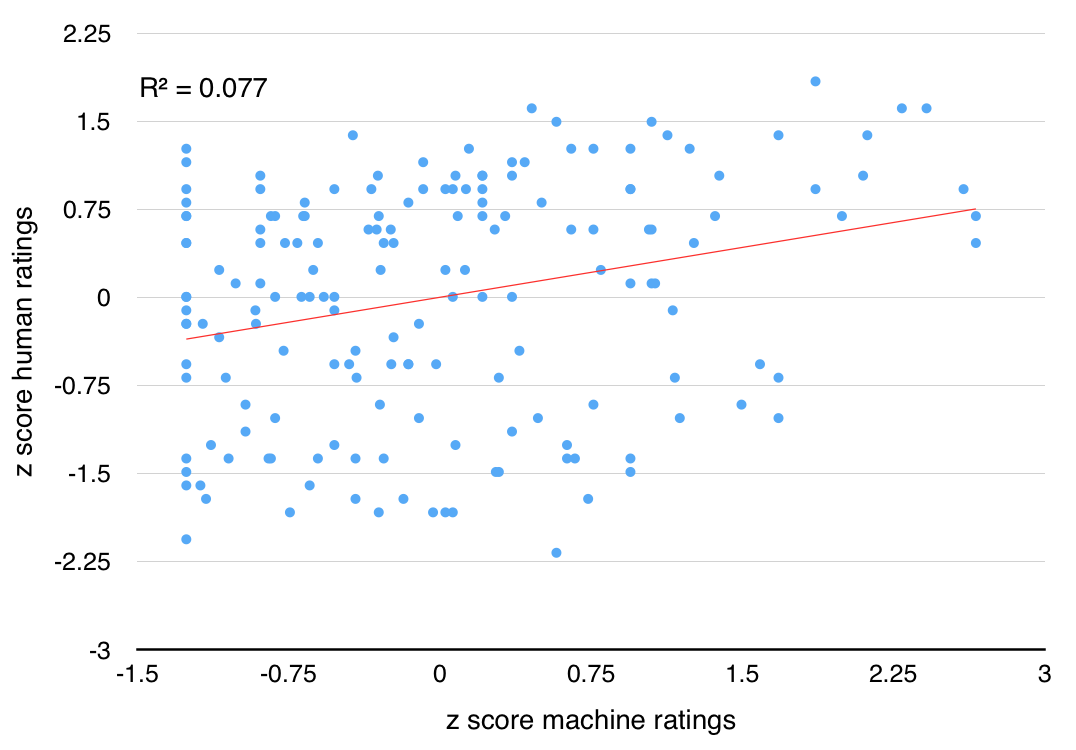
\includegraphics[width=0.8\textwidth]{extract_z_scores}
      \end{figure}

      Or the results can be presented like this:
      \begin{figure}[h]
        \caption{\textcolor{red}{group the human scores 1-5, then for each score plot the corresponding machine score in the box plot}}
        \centering
        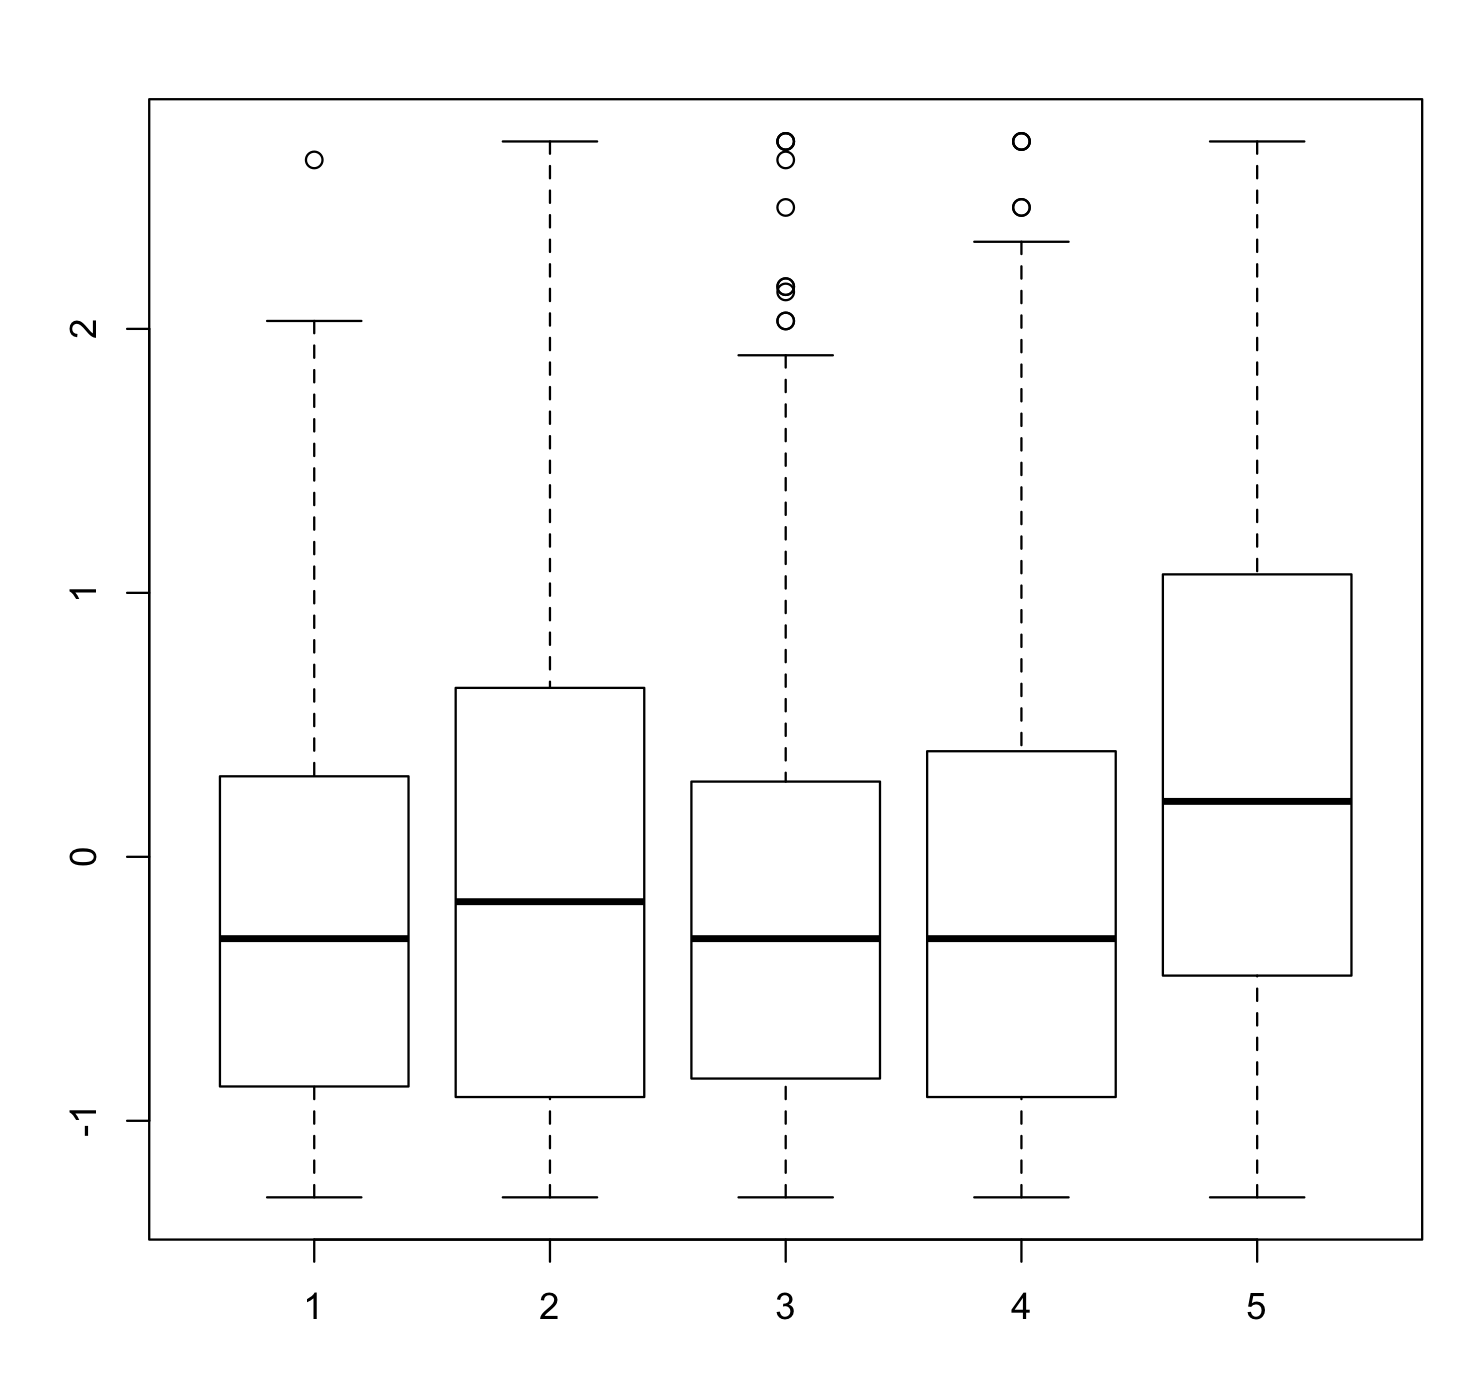
\includegraphics[width=0.8\textwidth]{boxplots}
      \end{figure}

      One selected extract \blockquote{As they pay income taxes} scored particularly poorly with a score of mean score of 2.2/5. Generally ratings correlate with the extract quality. These results are based on 1587 responses for 18 different clusters of extracts from six topics. The target population of this sample is all clusters of extracts selected for display in summaries.

      Regarding the results of the bigram vs. random summary comparison, there appeared was a preference for the bigram summary. 43\% of participants preferred the bigram summary, 20\% scored them the same and 34\% preferred the randomly generated summaries. Breaking this down by topic, the abortion bigram summary scored more than 5 times the random summary; for creation and healthcare both summaries scored equally. Interestingly, the random god summary scored higher than the accompanying bigram one.

      To test these results against \textbf{H3} we again used a one-sided Sign test. Excluding neutral ratings, the bigram model was successful 24/44 times. Based on this result we are unable to reject \textbf{H4}.

    \subsection{\textcolor{red}{TBD: Study 3: Section Comparison}}

  \section{Discussion}
    Based on on comments left as justification, some found the colors distracting and unnecessary as well as making the summary noisy and hard to read.
    Also need some samples of the comments that highlight interesting things

    On average, extracts scored well, showing pre-filtering is good at it's job.


    "Side [RANDOM] uses the scientific method and doesn't involve a fake diety at all in the science section." why god rand was better (also sentences made more sense)

\chapter{Summary \& Conclusion \label{chap:conclusion}}
  \section{Summary}
    In this project we have implemented a robust method for extracting points, a meaningfully shorter content unit than sentences. We make use of these in a summarization task by clustering points into cohesive sections. We then evaluate the effectiveness of our approach by comparing our summaries against those generated by a baseline statistical tool that uses sentence extraction.

    We were able to meet most of the project's initial goals. Using dependency parses, we have implemented a means of extracting more useful and complete points than those in previous project. We also improved on the detection of counter points by expanding the approach to account for antonyms --- rather than using negation terminology alone. While we also implemented an approach for the identification of co-occurring points, the results seem to be more variable and are highly dependent on large discussions where participants make many points.

    We opted to present the results of the analysis as summaries of the debate. Here we were able to go beyond our goals of counter/co-occurring points and include additional sections based on the points we had extracted. There are however areas that require further work. Results from our evaluation suggest that certain presentation decisions we not always popular. We also found that while scores allocated my our bigram model correlated with those of participants, this approach in selecting extracts from clusters was not significantly better than random when a compared at the summary level.

    The results of the summary comparisons were very positive with all our summary types performing significantly better in comparisons. We were able to reject our first two hypotheses. We were not able to reject \textbf{H3} but have gathered useful information for future work. We were unable to gather enough targeted feedback regarding sections to reject \textbf{H4} but again gathered much useful information for improving on the tool.

    Comments from study 3, at the social media workshop, suggested that the summaries fell between quantitative and qualitative analysis and this they could be made more useful by quoting the (already available) ratio of counter-point sides. Comments also suggested it would be useful to select the required summary length as well as provide links back to the input text. The disagreement section was referenced as being the most useful while participants found related points confusing.

  \section{Further Work}
    The implementation is still the product of an experimental development process. The components of the summary generation approach have poor maintainability. Next steps include reducing the agglomerative complexity and repetition as well as establishing a level of unit testing. Clearer definitions for the re-formatting of extracts and extract selection would also be beneficial for code readability. This ties into the corpus pre-processing and extract presentation, both areas that require a more integrated implementation.

    The tool chain is currently closely coupled with the corpus. We would like to establish a more less bespoke approach to make analysis of new corpora easier. One interesting direction would be a simple web application that capable of generating a summary for a discussion of the user's choosing from \textit{Reddit}, \textit{Hacker News} or online forum. This potential use case raises issue of the required discussion length. Currently a long discussion (upwards of 100,000 words) is required to extract a sufficient number of points to fill all our summary sections without repetition --- and build a good sample of counter/co-occurring points. This would likely require the summary structure to be more flexible, generating shorter summaries for shorter discussions and contextually removing sections where information was lacking.

    From the evaluation results we found that our bigram extract selection approach was not providing reliably better results than random --- though it's scores correlated with those of participants. This appeared to come down to both readability and informativeness. Currently extracts are weighted by the length, this is perhaps dominating the bigram score representing informativeness. It would also be interesting to introduce readability as an additional factor, perhaps by incorporating an \textit{Automated readability index}. Should the tool be made accessible to the public as a web application, there would also be the opportunity to use user rating of extracts to train a model for extract preference. The task of selecting readable, informative extracts that represent the cluster is an interesting task with various options for further work.

    Currently the approach models discussions as a flat list of posts --- without reply/response annotations. Using hierarchical discussion threads opens up interesting opportunities for Argument Mining using points extraction as a basis. A new summary section that listed points commonly made in response to other points in other posts would be an interesting addition. This would also be possible with discussions on \textit{Twitter} where reply information is also available. Related to this, adding user identity information would also make it possible to track a posts by the same user in discussions, and represents another interesting area for further features.

    Another direction that would be inserting to explore would be to build a graph-like representation of the discussion. Using point's subject and object information, a graph of nodes representing nouns connected by verbs as edges could be generated. This would be made more interesting if the semantic annotations from the verb frames could be included. As part of this project we experimented with a presentation of this type, an example is included in Appendix \ref{app:disc_graph}. Related to this is the possibility of using the semantic annotations in point frames to to investigate deeper abstractive summarization.

    There is also potential for further work on the summary presentation. Feedback gathered in Study 3 suggested that it would be useful to present the counts for negated points. This would allow the section to not only show a difference in opinion but to present how opinion is split. One comment suggested that the output was in between a quantitative and qualitative report and that adding more quantitative information to the summaries would make them more useful. Workshop attendees also suggested that being able to refer back to source text from the extracted points would also make the results more useful.

  \section{Conclusion}
    In this project we have shown that our points extraction is a viable foundation for summarization of online discussion. We think this success can be generalized to tasks beyond summarization that make use of text extracts. We have shown that existing tools struggle with the summarization of discursive text, and that our summaries with sections that are designed to give a more complete overview are preferred. Summarization is just one use case for such analysis and there are many other varied layers that could be built on top of our points extraction implementation.

    We see this project a step forward in the process of better understanding online discussion. Our hope is that this work can become the basis for further work and applications that allow the exploration of the wealth of ideas and arguments currently hidden in archived threads.


\appendix
\include{proof}

\bibliography{introduction,background,related}

\end{document}
